\chapter{Configuration et intégration}
\label{chap:chap_2}

\section{Configuration de Suricata}

\subsection{Vérification du chemin des règles}
Pour commencer, nous avons vérifié que le fichier \texttt{/etc/suricata/suricata.yaml} pointe bien vers le répertoire \texttt{/var/lib/suricata/rules}, et que le fichier \texttt{local.rules} est inclus dans la section \texttt{rule-files} :

\begin{verbatim}
$ grep -n "default-rule-path" /etc/suricata/suricata.yaml
2174:default-rule-path: /var/lib/suricata/rules

$ grep -A3 "rule-files:" /etc/suricata/suricata.yaml
2176:rule-files:
2177:  - suricata.rules
2178:  - local.rules
\end{verbatim}

\begin{figure}[H]
    \centering
    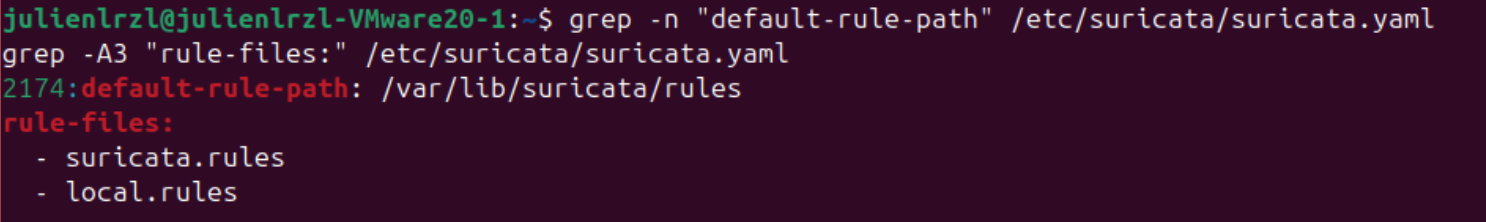
\includegraphics[width=0.9\linewidth]{assets/figures/suricata-rulefiles.png}
    \caption{Vérification du chemin des règles et inclusion de \texttt{local.rules}.}
\end{figure}

\subsection{Ajout d'une règle locale}
Une règle de détection ICMP a été ajoutée dans le fichier \texttt{local.rules} :

\begin{verbatim}
alert icmp any any -> any any (msg:"ICMP test detected"; sid:1000001; rev:1;)
\end{verbatim}


\begin{figure}[H]
    \centering
    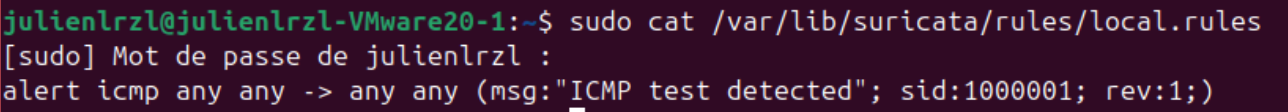
\includegraphics[width=0.9\linewidth]{assets/figures/local-rules.png}
    \caption{Règle ICMP de test ajoutée au fichier \texttt{local.rules}.}
\end{figure}

\subsection{Test de configuration}
Un test de configuration a permis de vérifier que le fichier YAML est valide et que les règles sont correctement chargées :

\begin{verbatim}
$ sudo suricata -T -c /etc/suricata/suricata.yaml
-- Configuration OK --
\end{verbatim}

\begin{figure}[H]
    \centering
    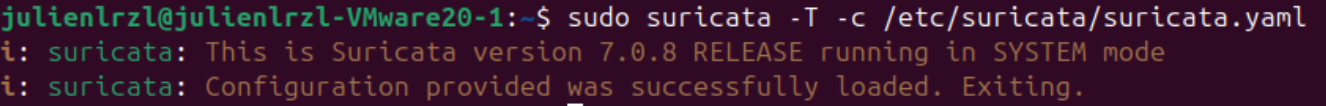
\includegraphics[width=0.9\linewidth]{assets/figures/suricata-test.png}
    \caption{Validation de la configuration de Suricata.}
\end{figure}

\subsection{Relance du service}
Suricata a ensuite été relancé en mode démon :

\begin{verbatim}
$ sudo pkill -9 suricata 2>/dev/null || true
$ sudo rm -f /var/run/suricata.pid
$ sudo suricata -c /etc/suricata/suricata.yaml -i ens160 -D
\end{verbatim}

\begin{figure}[H]
    \centering
    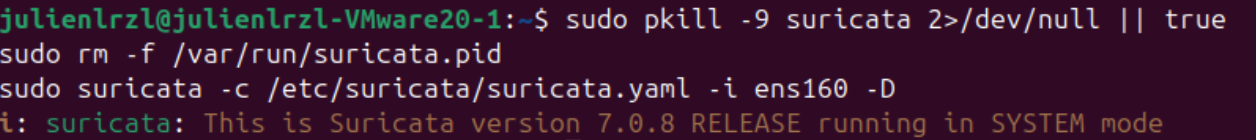
\includegraphics[width=0.9\linewidth]{assets/figures/suricata-restart.png}
    \caption{Relance de Suricata en mode démon sur l'interface \texttt{ens160}.}
\end{figure}

\subsection{Génération de trafic ICMP}
Un simple ping vers l’adresse publique de Google (8.8.8.8) a été utilisé pour générer du trafic ICMP :

\begin{verbatim}
$ ping -c 3 8.8.8.8
\end{verbatim}

\begin{figure}[H]
    \centering
    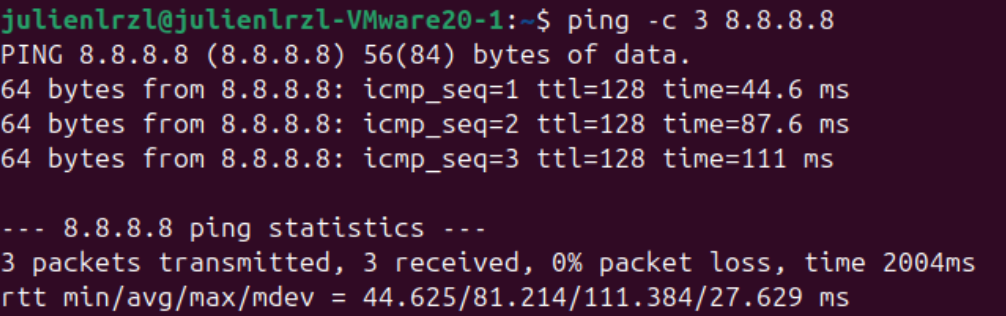
\includegraphics[width=0.9\linewidth]{assets/figures/ping-icmp.png}
    \caption{Génération de trafic ICMP avec la commande \texttt{ping}.}
\end{figure}

\subsection{Vérification des alertes générées}
L’analyse du fichier \texttt{/var/log/suricata/fast.log} montre bien que la règle locale a déclenché une alerte pour les paquets ICMP observés :

\begin{lstlisting}[style=bashstyle]
09/25/2025-18:16:40.523467 [**] [1:1000001:1] ICMP test detected [**] {ICMP} 172.16.150.130:8 -> 8.8.8.8:0
\end{lstlisting}


\begin{figure}[H]
    \centering
    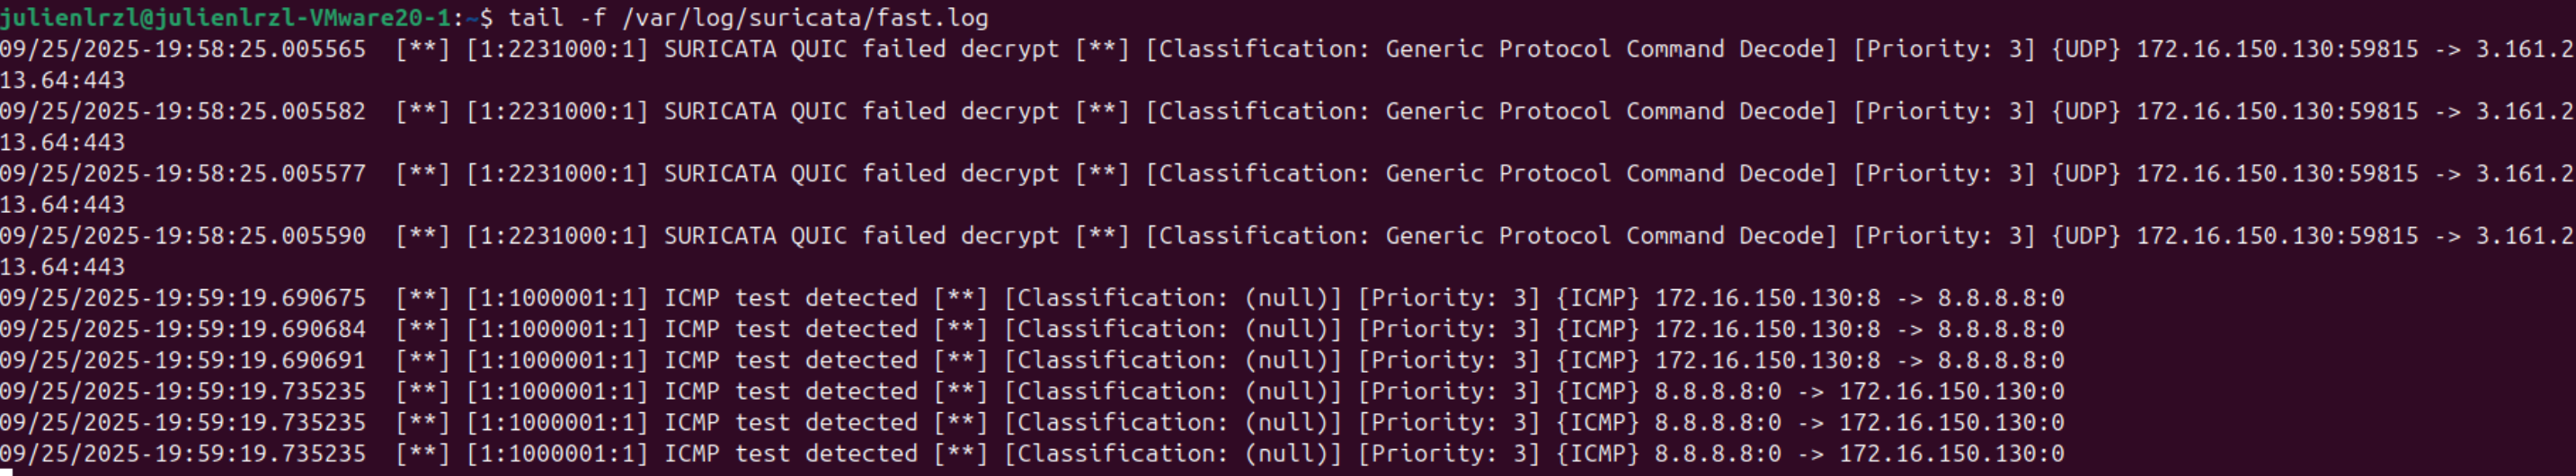
\includegraphics[width=0.9\linewidth]{assets/figures/icmp-alert.png}
    \caption{Alerte générée dans \texttt{fast.log} suite au ping ICMP.}
\end{figure}

\bigskip
En conclusion, Suricata est correctement configuré pour charger les règles locales et détecter du trafic ICMP simple, démontrant sa capacité à identifier des anomalies sur le réseau.